\documentclass{../template/labo}
\usepackage[utf8x]{inputenc}

\usepackage[frenchb]{babel}
\usepackage[T1]{fontenc}

\usepackage{graphicx}
\usepackage{amssymb}
\usepackage{amsmath}
\usepackage{wasysym} %smiley
\usepackage{hyperref}% hyperliens
\usepackage{tikz}
\usetikzlibrary{babel,positioning,calc}
%\usepackage[]{circuitikz}
\usepackage{textcomp}
% \usepackage{minted}
\usepackage[long]{datetime}
\usepackage{gensymb} % \ohm, celsius
\usepackage{framed}
\usepackage{pdfpages}
\usepackage{todo}
\usepackage{paralist}
\usepackage{multicol}

\usepackage{mathastext} % math as standfard text : units are respecting typography conventions.
\usepackage{fancyhdr} %en-tête
\usepackage{qrcode}




\usepackage{xspace} % typographie IN
\usepackage{hyperref}% hyperliens
\usepackage[all]{hypcap} %lien pointe en haut des figures
\usepackage[french]{varioref} %voir x p y
\usepackage{fancyhdr}% en têtes
%\input cyracc.def
\usepackage{pgfplots}
\usetikzlibrary{babel,positioning,calc}
\usepackage[americanresistors ]{circuitikz}
%\usepackage[]{gnuplottex}
\usepackage{ifthen}

\usepackage[]{pdfpages}
\usepackage[]{subfig}
\usepackage[]{attachfile}

% \langexam{frenchb}

\newboolean{koriG}
\ifx\koriG\undefined
\correction{false}
\else
\correction{true}
\fi

% \correction{false}
 %\correction{true}

\author{The Fantastic Four}


%% fancy header & foot
\pagestyle{fancy}
\lhead{[ELEC-H-301] Électronique appliquée\\ LABO \no 3 : Diodes et alimentations\ifthenelse{\boolean{corrige}}{~-- corrigé}{}}
\rhead{v1.0.2\\ page \thepage}
\cfoot{}
%%

\pdfinfo{
/Author (Raoul Sommeillier, ULB -- BEAMS)
/Title (LABO 3 ELEC-H-301, Diodes et alimentations)
/ModDate (D:\pdfdate)
}

\hypersetup{
pdftitle={LABO 3 [ELEC-H-301] Électronique appliquée: Diodes et alimentations},
pdfauthor={Raoul Sommeillier, 2017 ULB - BEAMS  },
pdfsubject={Filtrage}
}

%\date{\vspace{-1cm}\mydate\today}
%\title{\vspace{-2cm} Labo \no 6\\ Électronique appliquée [ELEC-H-301]\\Réalisation d'un ampli à transistor\ifthenelse{\boolean{corrige}}{~\\Corrigé}{}}

%\author{\vspace{-1cm}}%\textsc{Yannick Allard}}

\setlength{\parskip}{0.5cm plus4mm minus3mm} %espacement entre §
\setlength{\parindent}{0pt}


\begin{document}

\tptitle{}{Séance 3~: Diodes et alimentations}

\section{Introduction}

\section{But de la manipulation}
Cette manipulation a pour but d'illustrer :
\begin{itemize}
\item au niveau «application» : le fonctionnement d'une alimentation AC/DC linéaire
\item au niveau «composant» : le fonctionnement des diodes les plus courantes : diode à jonction PN, diode Zener, LED.
\end{itemize}

\section{Prérequis}
\begin{itemize}
\item Circuit RC du premier ordre
\item Chapitre \no 17 du livre de référence (ed 5).\\ En particulier :
\begin{itemize}
\item rôle des diodes (redressement) dans les alimentations
\item redresseurs simple et double alternance
\item polarisation d'une diode
\item diode Zener
\item diode LED
\end{itemize}


%\item Être capable de calculer un gain et une résistance de sortie en utilisant un schéma équivalent.
%\item Être capable de tracer un diagramme de Bode.
%\item Avoir compris les principes de la polarisation.

\end{itemize}

\subsection{Prédéterminations}
Toutes les sections «prédétermination» ainsi que les questions~\ref{Q:7} à~\ref{Q:9} et~\ref{Q:22} doivent être faites \textbf{avant} l'arrivée au laboratoire.

Le TP 4 portant sur les diodes fait également office de prédéterminations.
%Les prédéterminations des questions \ref{Q:1} à \ref{Q:predet} 


\subsection{Objectifs}
À la fin de ce laboratoire, vous devez être capable :
\begin{itemize}
\item de maîtriser le circuit d'une alimentation AC/DC classique,
\item d'expliquer le fonctionnement du pont de diodes,
\item de prévoir l'effet d'une charge sur l'alimentation,
\item de dimensionner la capacité de sortie pour un \textit{ripple} donné en faisant les hypothèses appropriées ;
\item de calculer un régulateur de tension à diode Zener (courant, puissance, rendement, etc) ;
\item d'expliquer le fonctionnement des circuits comprenant des diodes (à jonction, LED, Zener, etc) ;
\item de lire la notice d'une diode et d'en extraire les informations utiles ;
\item d'utiliser la caractéristique d'une diode;
\item de dimensionner une résistance de limitation de courant pour une LED ;
\end{itemize}
%\clearpage
\newpage
\pagestyle{fancy}
%\begin{Q}
%	À quelle condition cette source est-elle linéaire ?
%	\label{Q:1}
%	\reponse{$g$ doit être constant.}
%\end{Q}

\section{Concepts}
Les circuits électroniques ont besoin d'être alimentés par des sources de tension continue. Dans la plupart des cas, l'amplitude de ces tensions d'alimentation doit être de l'ordre de quelques volts ou quelques dizaines de volts (les plus courantes sont $2.5V$, $3.3V$, $5V$, $12V$ et $15V$).
Malheureusement, le réseau électrique nous fournit une tension sinusoïdale de $220V_{eff}$. Il est donc nécessaire de transformer cette tension alternative en tension continue de plus faible amplitude ; c'est le rôle des alimentations AC/DC.
Toute alimentation de ce type doit entre autres réaliser un "redressement" des grandeurs électriques, ce qui se fait en pratique au moyen d'une ou plusieurs diodes.
 
Dans la suite, nous appellerons :%\marginpar{mettre ça plus loin ?}
\begin{itemize}
\item source, le réseau 220V (tout ce qui se trouve derrière la prise) ;
\item alimentation, le circuit que nous allons étudier ;
\item charge, le montage électronique qui doit être alimenté par notre alimentation. Durant la manipulation, nous simulerons la charge par une résistance consommant la puissance désirée, équivalent de Thévenin.
\end{itemize}

Commençons par comprendre le fonctionnement et l'utilisation d'une diode.

\section{Polarisation d'une diode, exemple de la LED}
Dans cette section, nous allons nous intéresser à la polarisation d'une diode afin de faire le lien entre les caractéristiques théoriques et l'utilisation pratique d'une diode.
\subsection{Caractéristique I/V théorique}
\subsubsection{Conventions}
Les conventions pour le tracé de caractéristique I/V pour les diodes sont «courant positif de l'anode vers la cathode, convention récepteur» :
\begin{figure}[h!]
	\begin{center}
		\begin{circuitikz}\draw
			(0,0) node[anchor=east] {A} to [short,i>^=$I$] (1.5,0)
			(0,0) to [Do, v<=$V$] (2.5,0) node [anchor=west]{K}
		;\end{circuitikz}
	\end{center}
\caption{Conventions électriques}
\label{fig:source}
\end{figure}

\marginpar{\color{white}6dd9a4cc75f4c05c00780b57a702246076eeab706d614a915428c03372ddf7ad445c006d38cedcd6a4749e838125d94a3fdff36a9131771074bc3c98df9b11c6}
%\ifthenelse{\boolean{corrige}}{Bonus : Quelle(s) diodes ont permis à leur inventeur(s) d'obtenir un prix Nobel ?}{Bonus : Quelle(s) diodes ont permis à leur inventeur(s) d'obtenir un prix Nobel ?}
%et une petite citation par ici\dots
%QR diode
%QR LED
%QR pont
%QR blague
\begin{figure}[h!]
	\vspace{-0.5cm}
	\begin{center}
		%\subfloat[Préemption avec invalidation de la mémoire cache]{\label{fig:preemption_cacheinv}\includegraphics[width=8.5cm]{figures/preemption-crop.pdf}}%\hspace*{0.5cm}
		\subfloat[TLHR5401]{\href{http://www.vishay.com/docs/83012/tlhg540.pdf}{
\includegraphics[width=2.7cm]{figures/QR_LED.pdf}}}\hspace{0.5cm}
		\subfloat[1N5392]{\href{http://www.protostack.com/download/1N5391-9.pdf}{
\includegraphics[width=2.7cm]{figures/QR_1N5392.pdf}}}\hspace{0.5cm}
		\subfloat[Pont de Graetz]{\href{http://diotec.com/tl_files/diotec/files/pdf/datasheets/b40c2300}{
\includegraphics[width=2.7cm]{figures/QR_PONT.pdf}}}\hspace{0.5cm}
		\subfloat[{\tiny «Electronique», \textit{Fantøme}}]{\hspace{0.cm}\href{https://www.youtube.com/watch?v=sAWEYLPyovA}{
\includegraphics[width=2.7cm]{figures/QR_Fantome.pdf}}\hspace{1.25cm}}
		%http://diotec.com/tl_files/diotec/files/pdf/datasheets/b40c2300
	\end{center}\vspace{-0.5cm}
\caption{QR codes cliquables vers la documentation des composants}
\label{fig:}
\end{figure}
%{TLHR5401}
%\begin{center}
%\ifthenelse{\boolean{corrige}}{\includegraphics[height=3.5cm]{Fred_Stiller.jpeg}}{\includegraphics[height=2.5cm]{Fred_Stiller.jpeg}}
%\end{center}

\newpage
\subsubsection{Caractéristique I/V}
La caractéristique courant--tension théorique de la LED ressemble à la Figure~\ref{fig:carac_LED} :
\begin{figure}[h!]
	\vspace{-0.5cm}
	\begin{center}
	\ifthenelse {\boolean{corrige}} {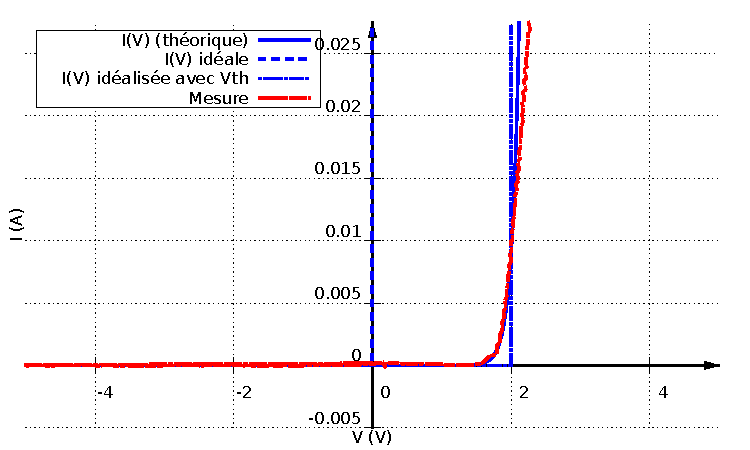
\includegraphics[width=\linewidth]{mesures/carac_mes.pdf}} {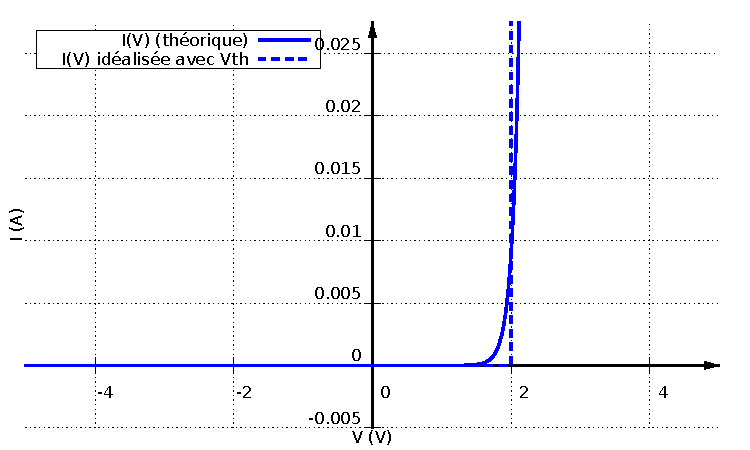
\includegraphics[width=12cm]{figures/carac.pdf}}
	\end{center}\vspace{-0.5cm}
\caption{Caractéristique I/V de la LED}
\label{fig:carac_LED}
\end{figure}	

\subsection{Mesure de points de fonctionnement}
Soit le montage de la Figure~\vref{fig:circuit_led}.
\begin{figure}[h!]
	\begin{center}
	\shorthandoff{:!}
		\begin{circuitikz}\draw
			(0,0) to [battery, l=$V_{dc}$] (0,3)
			to [european resistor, l=$R$] (3,3)
			to [leDo] (3,0) -- (0,0)
		;\end{circuitikz}
	\shorthandon{:!}
	\end{center}
\caption{Diode polarisée en direct si $V_{dc}>0$}
\label{fig:circuit_led}
\end{figure}

	
\textit{Cette partie du laboratoire est à réaliser sur le protoboard en utilisant l'alimentation continue $5V$.}
	
\Question
{
	En prenant $R=\lbrace 100, 330, 1000, \infty \rbrace \Omega$ et la tension de seuil indiquée dans la documentation de la LED \href{http://www.vishay.com/docs/83012/tlhg540.pdf}{TLHR5401} ($V_F$), mesurez et placez les 4 points correspondants sur le graphe de la Figure~\vref{fig:carac_LED}. Utilisez le protoboard et $V_{dc}=5V$.
}
{Voir graphe.}%R
	\label{Q:1}

\Question
{
	L'approximation I(V) idéalisée avec seulement la tension de seuil est-elle une bonne approximation ?
}
{Oui}%R
	\label{Q:2}

\Question
{
	Indiquez l'état de la diode sur le graphe de la page précédente en fonction de I.
}
{}
	\label{Q:3}
	
\Question
{
	En tenant compte de la réponse à la question~\ref{Q:2}, calculez la valeur de $R$ pour obtenir un courant de 20mA dans la LED.	
}
{$$R=\frac{V_{dc}-V_{th}}{I_D}=150\Omega$$}%R
	\label{Q:4}

\Question
{
	Que se passe-t-il si la diode est mise en inverse ($V_{dc}<0V$ ou diode inversée) ?  Que peut on dire du courant la traversant (faire une mesure) ? Est-elle éclairée ?
}
{La led est en inverse et est éteinte. Le courant la traversant est très faible : $\approx 50\mu A$ }%R
	\label{Q:5}

\Question
{
	Quelles précautions doivent être prises lors du fonctionnement en direct ? Même question pour un fonctionnement en inverse.
}
{Le courant maximum ne doit pas être dépassé. En inverse, la tension de claquage ne doit pas être atteinte}%R
	\label{Q:6}


%Vcc/R/LED

%Pour R=330, 1k, 3k,Vcc=5/-5V relever I et V et placer les points sur le graphe précédent

%Le modèle 
%\newpage
\section{Structure d'une alimentation AC/DC}
Il existe plusieurs types d'alimentations AC/DC. Le type le plus simple (l'alimentation linéaire) possède la structure suivante:

\begin{figure}[h!]
	\begin{center}
		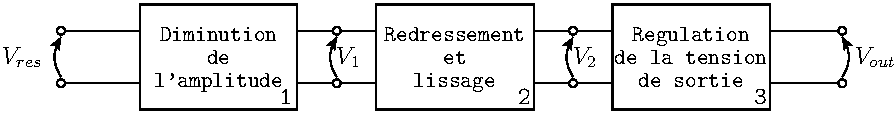
\includegraphics[width=\linewidth]{figures/alim.pdf}
	\end{center}
\caption{Structure d'une alimentation linéaire}
\label{fig:alim}
\end{figure}

On peut diviser l'alimentation en 3 étages, remplissant chacun une fonction :
\begin{itemize}
\item Le \textbf{1\ier étage} a pour but de diminuer l'amplitude de la tension alternative, pour la rendre compatible avec les besoins de la charge. Pour cela, on utilise un transformateur abaisseur de tension.
Dans ce labo, nous utiliserons un transformateur $220V/9V$.
Le transformateur a un avantage supplémentaire : il assure une isolation galvanique entre la charge et la source, ce qui garantit une certaine sécurité à l'utilisateur, même en cas de défaut de l'alimentation.
A la sortie du 1\ier étage, on a une tension ($V1$) toujours sinusoïdale, mais d'amplitude plus faible, convenant mieux à notre application.

\item Le \textbf{2\ieme étage} a pour but de transformer cette tension ($V1$) alternative en une tension continue. Pour cela, il combine 2 fonctions : le redressement et le lissage.
Le redressement a pour but de transformer une tension purement alternative (sans composante continue) en une tension unipolaire (c'est à dire toujours positive). Il existe deux types de redressement : le simple redressement et le double redressement; nous utiliserons le double redressement.
Le lissage a pour but d'atténuer la partie alternative de la tension redressée, pour rendre celle-ci principalement continue.
Dans la pratique, on aura une tension $V2$ qui sera la somme d'une composante continue (qui est celle qui nous intéresse) et d'une composante alternative non sinusoïdale résiduelle, le \textit{«ripple»}, de faible amplitude.

\item Le \textbf{3\ieme étage} a pour but de réguler l'amplitude de la tension de sortie. En effet, la tension $V2$ n'est pas parfaitement continue, de plus, l'amplitude de sa composante continue dépend de celle de la source, qui peut fluctuer fortement ($\pm10\%$\footnote{La tension du réseau peut avoir une telle variation, demandez à M. Maun.}). %\marginpar{renommer correctement V1/2/out}
Il existe plusieurs façons de réaliser cet étage ; dans ce labo, nous étudierons le plus simple, basé sur une diode Zener.
\end{itemize}


\newpage
\section{Redressement simple alternance}
Nous allons nous intéresser au deuxième étage de l'alimentation.

\textit{Cette partie du laboratoire est à câbler sur le protoboard. Alimentez votre montage avec le transformateur \textbf{sans utiliser les bornes d'alimentation du protoboard}.}

Voici le schéma d'un redresseur simple alternance :
\begin{figure}[h!]
	\begin{center}
		\begin{circuitikz}\draw
			(0,0) to [sV, l=$V_{ac}$] (0,3)
			to [Do] (3,3)
			to [european resistor,l_=$Z_{Charge}$] (3,0) to (0,0)
			(3.5,3) to [open, v^<=$V_{charge}$] (3.5,0)
		;\end{circuitikz}
	\end{center}
\caption{redresseur simple alternance}
\label{fig:source}
\end{figure}

\Question
{
	Tracez l'allure du courant circulant dans le circuit en fonction du temps.
}
{Courbe rouge $I_{ch}$\\
	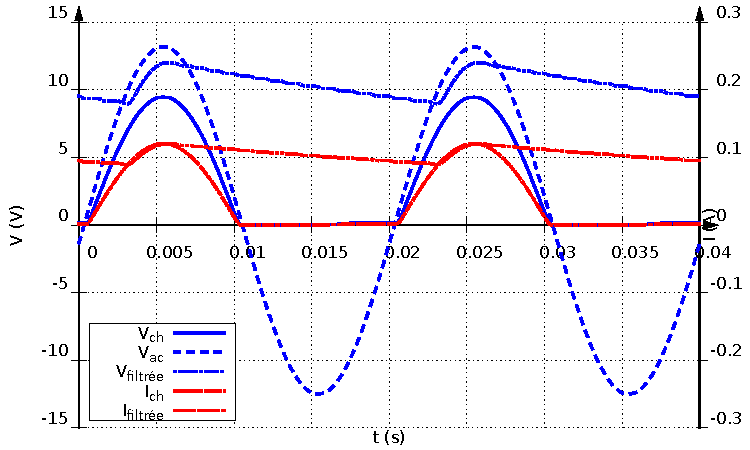
\includegraphics[width=\linewidth]{mesures/simple_alternance.pdf}}%R
	\label{Q:7}

\Question
{
	Tracez sur un même graphe la tension aux deux bornes de la diode. Précisez l'état de la diode. Utiliser une tension de seuil de 1V pour simplifier (\textit{cf} \href{http://www.protostack.com/download/1N5391-9.pdf}{documentation 1N5392}).%\marginpar{donner un graphe ???}
}
{Courbes $V_{ac}$ et $V_{ch}$ du graphe précédent.}%R
	\label{Q:8}

\Question
{
	La tension de sortie est-elle stable ? Que proposez-vous comme solution pour augmenter cette stabilité ?
}
{Non, ajouter une capacité de filtrage.}%R
	\label{Q:9}


\section{Filtrage capacitif}
Effectuons un filtrage capacitif\footnote{Il est également possible d'effectuer un filtrage inductif pour limiter l'amplitude des pics de courant sur la source alternative mais ces phénomènes dépassent les limites de ce cours.} en ajoutant une capacité en parallèle avec la charge.
\begin{figure}[h!]
	\begin{center}
		\begin{circuitikz}\draw
			(0,0) to [sV, l=$V_{ac}$] (0,3)
			to [Do] (5,3)
			to [european resistor,l=$R_{Ch}$] (5,0) to (0,0)
			(4,3) to [eC,l_=$C$, *-*] (4,0)
			(6,3) to [open, v^<=$V_{charge}$] (6,0)
		;\end{circuitikz}
	\end{center}
\caption{redresseur simple alternance}
\label{fig:source}
\end{figure}

\subsection{Prédéterminations}
\Question
{
	Justifiez la polarité utilisée pour la capacité.
}
{Redresseur simple alternance, tension positive à la cathode/ rapport à la charge.}%R
	\label{Q:10}

\Question
{
	%Q
	Tracez l'allure de $V_{charge}$ en tenant compte de la capacité.
}
{Voir graphe précédent, $V_{filtrée}$}%R
	\label{Q:11}

\subsection{Manipulation}
\Question
{
	Tracez l'allure du courant circulant dans la charge. Indiquez les intervalles de charge et de décharge.
}
{Voir graphe précédent, courbe rouge $I_{filtrée}$}%R
	\label{Q:12}


\Question
{~\\
\begin{itemize}
\item Vérifiez expérimentalement. (\textbf{ATTENTION} à la polarité de votre condensateur).
\item Placez une résistance de charge en parallèle avec le condensateur ; observez son effet sur $V_{charge}$ pour différentes valeurs.
\item Expliquez qualitativement l'influence de cette résistance sur l'allure de $V_{charge}$.
\item Remarquez que le signal comporte plusieurs «phases» successives.
\item Quelle est la forme d'onde dans chacune de ces phases ?
\end{itemize}
}
{}%R
	\label{Q:13}


\subsection{Calcul de l'ondulation}
On remarque que lorsque le circuit est chargé, la tension de sortie ondule. Quantifions cette ondulation en fonction des éléments du circuit.

La tension de sortie peut être décomposée en une composante continue et une composante alternative, d'où : $V=V_m+\Delta_V$

\Question
{
	Établissez une formule permettant d'estimer $\Delta_V=f(R,C, V_m,\dots)$. %\marginpar{manque ptet qques paramètres}
	
	Utilisez les approximations suivantes :
	\begin{itemize}
	\item $\Delta_V<<V_m$
	\item le temps de charge du condensateur est négligeable devant son temps de décharge.
	\item la décharge de la capacité est linéaire
	\end{itemize}
}
{}%R
	\label{Q:14}


Cette formule permet de dimensionner la valeur de la capacité à utiliser pour lisser la tension de sortie pour limiter l'ondulation à une valeur donnée pour une charge donnée.

\Question
{
	Mesurez $\Delta_V$ et comparez à la valeur calculée pour les mêmes paramètres. L'approximation faite est-elle valable, optimiste ou pessimiste ?
}
{}%R
	\label{Q:15}

\newpage
\section{Redressement double alternance}
Le redresseur simple alternance a le défaut majeur de ne redresser qu'une seule alternance (et également de consommer un courant continu sur le réseau alternatif\footnote{Pour s'en rendre compte, effectuez une transformée de Fourier du courant délivré par la source ou calculez sa valeur moyenne. La circulation de courant continu sur un réseau alternatif pose un certain nombre de problèmes détaillés dans les différents cours de M. Maun.}).

Ce défaut peut être corrigé et le courant fourni par le réseau peut être alternatif si la deuxième alternance du signal est mise à contribution. Un redresseur double alternance\footnote{Le pont redresseur à 4 diodes est aussi appelé «Pont de Graetz»}  aura également moins d'ondulation.

\textit{Cette partie du laboratoire est à réaliser avec les composants sur support. Alimentez votre montage avec le transformateur.}

%\newpage
Voici le schéma électrique d'un redresseur double alternance :
\begin{figure}[h!]
	\begin{center}
		\begin{circuitikz}\draw
			(-2,1) to [sV, l_=$V_{ac}$] (-2,3)
			(-2,1) to (-1,1) to (-1,1.75) to [short,-*](2,1.75)
			(-2,3) to (-1,3) to (-1,2.25) to [short,-*](0,2.25)
			(0,0) to [Do] (0,2) to [Do](0,4)
			(2,0) to [Do,*-] (2,2) to [Do, -*](2,4)
			(0,4) to [short](5,4)
			(0,0) to [short](2,0)
			(5,4) to [european resistor,l=$Z_{Ch}$] (5,0) to (2,0)
			(4,4) to [eC,l_=$C$, *-*] (4,0)
			(6,4) to [open, v^<=$V_{charge}$] (6,0)
		;\end{circuitikz}
	\end{center}
\caption{redresseur double alternance}
\label{fig:source}
\end{figure}	
	
	\subsection{Prédéterminations}
\Question
{
			Expliquez pourquoi il n'est \textbf{pas} possible de mesurer $V_{ac}$ et $V_{charge}$ en même temps avec un oscilloscope à deux canaux non isolés ?
			Justifier en quoi cela pourrait endommager le circuit ?%\footnote{Nous rappelons à nos aimables lecteurs que cette question a inspiré un certain nombre de questions d'examens et que l'assistant qui les écrit a encore pas mal d'idées à utiliser.} ?
}
{}%R
	\label{Q:16}
	
\Question
{
	Expliquez les avantages de ce circuit par rapport au précédent.
}
{}%R
	\label{Q:17}

\Question
{
	Tracez l'allure de la tension de sortie avec et sans capacité de filtrage.
}
{}%R
	\label{Q:18}

\Question
{
	Tracez l'allure de la tension aux deux bornes d'une diode et déduisez-en son état en fonction du temps.
}
{}%R
	\label{Q:19}


\Question
{
	Que devient la formule d'approximation déterminée à la question~\ref{Q:ondulation} ? 
}
%	Vérifiez expérimentalement.
{}%R
	\label{Q:20}


%\subsection{Manipulation}
%\Question
%{
%	Vérifiez expérimentalement les trois résultats précédents.
%}
%{}%R
%	\label{Q:21}
%
%
%\newpage
%\section{Régulation à diode Zener}
%Le circuit précédent produit une tension quasiment continue mais dont l'amplitude n'est pas précisément connue et peut varier assez fortement ($\pm 10\%$). Nous devons maintenant la réguler afin d'obtenir une tension continue de valeur connue indépendante des variations du réseau. Nous allons utiliser une diode Zener. D'autres composants permettant d'effectuer des régulations plus précises existent.
%
%\subsection{La diode Zener}%{\color{white}, sa vie, son œuvre\dots}
%
%La diode Zener utilise le phénomène d'avalanche existant d'une diode\footnote{Le phénomène d'avalanche n'est destructeur que si la température limite de jonction de la diode est atteinte. Généralement, l'entrée en avalanche donne lieu à la circulation d'un courant qui va échauffer très rapidement la diode et la détruire lorsque la température limite de jonction aura été atteinte.} dont le seuil a été fixé à la fabrication de la diode. Notez qu'une diode Zener  se comporte comme une diode classique si elle est utilisée en direct. Au risque de répéter un point important, une diode Zener s'utilise en \textbf{inverse} car sa caractéristique intéressante est son phénomène d'avalanche (en inverse).
%
%Les conventions électriques utilisées pour la diode Zener sont les mêmes que pour toute diode, pour rappel, 
%\begin{figure}[h!]
%	\begin{center}
%		\begin{circuitikz}\draw
%			(0,0) node[anchor=east] {A} to [short,i>^=$I$] (1.5,0)
%			(0,0) to [zDo, v<=$V$] (2.5,0) node [anchor=west]{K}
%		;\end{circuitikz}
%	\end{center}
%	\vspace{-0.4cm}
%\caption{Conventions électriques}
%\label{fig:zenerconv}
%\end{figure}
%\vspace{-0.4cm}
%sa caractéristique comporte un coude supplémentaire en inverse :
%\begin{figure}[h!]
%	\begin{center}
%		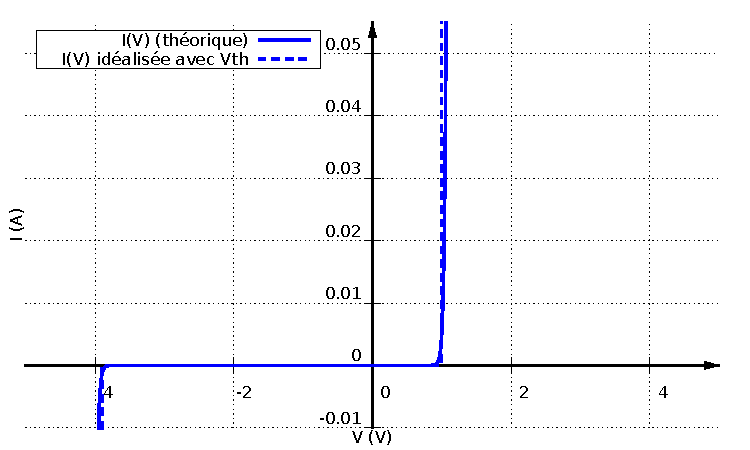
\includegraphics[width=10cm]{figures/carac_zener.pdf}
%	\end{center}
%\caption{Caractéristique I/V de la diode Zener}
%\label{fig:carac_Zener}
%\end{figure}
%
%Notez que la tension de Zener est positive et que sur la caractéristique, le phénomène d'avalanche se produit pour $V=-V_z$. Il faut donc utiliser la diode Zener en \textbf{inverse} pour pouvoir utiliser l'effet Zener. En direct, une diode Zener se comporte comme une diode commune ayant une tension de seuil de $0.7V$ généralement.
%
%\subsection{Utilisation en avalanche}
%Intéressons-nous uniquement à l'étage de régulation de l'alimentation présentée Figure~\vref{fig:alim} dans un premier temps.
%
%Soit le circuit de la Figure~\vref{fig:regulateur}.
%\begin{figure}[h!]
%	\begin{center}
%		\begin{circuitikz}\draw
%			(0,0) to [battery, invert, l=$V_{2}$] (0,3)
%			to [european resistor,l=$R$] (3,3)
%			(3,0) to [zDo, i<=$I_z$] (3,3)
%			(3,0) to (0,0)
%			(3,0) to [short,*-o] (4,0)
%			(3,3) to [short,*-o] (4,3)
%			(4,3) to [open,v^<=$V_{out}\equiv -V(Fig\ref{fig:zenerconv})$] (4,0)
%		;\end{circuitikz}
%	\end{center}
%\caption{Diode Zener utilisée en avalanche pour effectuer une régulation en tension}
%\label{fig:regulateur}
%\end{figure}

\Question
{
	En supposant $V_2>V_{out}$, prédéterminez :
	\begin{itemize}
	\item l'état de la diode Zener
	\item la tension $V_{out}$
	\item la valeur du courant traversant la diode $I_z$ %\marginpar{ajouter $I_z$ aux circuits}
	\item les valeurs des puissances dissipées par les différents éléments du circuit
	\end{itemize}
}
{}%R
	\label{Q:21}


\subsection{Influence d'une charge}
Ajoutons une charge à ce beau circuit, nous obtenons :
\begin{figure}[h!]
	\begin{center}
		\begin{circuitikz}\draw
			(0,0) to [battery, v=$V_{2}$] (0,3)
			to [european resistor,l=$R$] (3,3)
			(3,0) to [zDo, i<=$I_z$] (3,3)
			(3,0) to (0,0)
			(3,0) to [short,*-o] (4,0) to (5,0)
			(3,3) to [short,*-o] (4,3) to [short, i=$I_{out}$] (5,3)
			(5,3) to [european resistor,l=$R_{\mbox{ch}}$] (5,0)
			(3.5,3) to [open,v^<=$V_{out}$] (3.5,0)
		;\end{circuitikz}
	\end{center}
\caption{Circuit de régulation de tension, chargé}
\label{fig:regul_charge}
\end{figure}

\newpage
\subsection{Prédéterminations}
%Le circuit alimente une charge qui consomme $I_{out}$.
%Sachant que :

\begin{itemize}
\item $V_2 = 13V$
\item $V_z = 9.1V$
\item la puissance maximale que peuvent dissiper $R$ et la diode est $1W$.
\end{itemize}
%\subsubsection{Cas limites}
\Question
{
	Indiquez l'état de la diode, exprimez et calculez $I_{\mbox{out}}$ et la puissance dissipée par les différents éléments ($R, D, R_{\mbox{ch}}$) dans les 3 cas suivants :
	\begin{itemize}
	\item la charge est un court-circuit
	\item la charge est un circuit ouvert
	\item la charge est telle que le courant circulant dans la diode est négligeable devant les autres courants circulant dans le circuit.
	\end{itemize}
}
{
	\begin{itemize}
		\item CC : $P_{\mbox{charge}}=0$, $P_R=V_2^2/R$, $P_D=0$, la diode est bloquée
		\item CO :  $P_{\mbox{charge}}=0$, $P_R=\left(V_2-V_z\right)^2/R$, $P_D=V_z\cdot \left(V_2-V_z\right)/R$, la diode est passante en inverse
		\item $I_D\#0$ : $P_{\mbox{charge}}=V_z\cdot \left(V_2-V_z\right)/R$, $P_R=\left(V_2-V_z\right)^2/R$, $P_D\#0$, la diode est passante en inverse (mais à la limite)
		\end{itemize}	
	}%R
	\label{Q:22}

\Question
{
	%Calculez les valeurs numériques correspondant aux 3 cas de la question~\ref{Q:23b}. 
	$R$ et $D$ ne doivent pas dissiper plus que leur puissance maximale admissible quelque soit la charge. %, cela revient à choisir le cas le plus contraignant.
	\begin{itemize}
	\item Pour quelle valeur de $I_{out}$ la puissance dissipée par la diode est-elle maximale ?
	\item Pour quelle valeur de $I_{out}$ la puissance dissipée par la résistance $R$ est-elle maximale ? 
	\item Déduire la valeur minimale de $R$ des 2 calculs précédents (tous les composants doivent survivre).
	\item Quel est le courant maximum que ce circuit peut fournir à la charge (en méritant encore son nom, \textit{i.e.} avec une tension de sortie régulée) ?
	\item Quelle est la résistance de charge correspondante ?
	\end{itemize}
}
{}%R
	\label{Q:23}

\Question
{
	%Q
	Déduisez-en la caractéristique $V_{out} = f(I_{out})$ du montage.
	%
	Justifiez l'appellation «régulateur de tension» de ce circuit.
}
{}%R
	\label{Q:24}

%
%\begin{Q}
%	%Discutez les états possibles de la diode en fonction de la valeur de $I_{out}$. $I_{out}$ peut varier de $0$ à une valeur maximale à déterminer dépendant de $R$.
%	
%	
%	
%	
%	\label{Q:25}
%	\reponse{}%R
%\end{Q}
%\subsubsection{Choix de design}
%\begin{Q}
%	
%	\label{Q:24}
%	\reponse{}%R
%\end{Q}
%
\Question
{
	Établissez l'expression du rendement du montage en fonction de $I_{out}$.
	%
	Discutez le résultat obtenu.
}
{}%R
	\label{Q:25}

\vspace{-0.5cm}
%
%
%\begin{Q}
%	Déterminez la valeur de R permettant de fournir la puissance la plus grande possible à la charge.
%	
%	
%	Quelle est alors la résistance de charge minimum que ce circuit peut alimenter correctement ?
%	\label{Q:26}
%	\reponse{}%R
%\end{Q}
\subsection{Manipulation}
\Question
{
	Ajoutez le régulateur de tension à la sortie de votre montage.
}
{}%R
	\label{Q:26}

\Question
{
	Tracez la caractéristique de sortie du circuit en relevant les points de fonctionnement pour différentes valeurs de résistance de charge. Comparez avec vos prédéterminations.
}
{}%R
	\label{Q:27}

\Question
{
	Quel est le prénom de Zener ? Quel est le prénom de Graetz ?
%	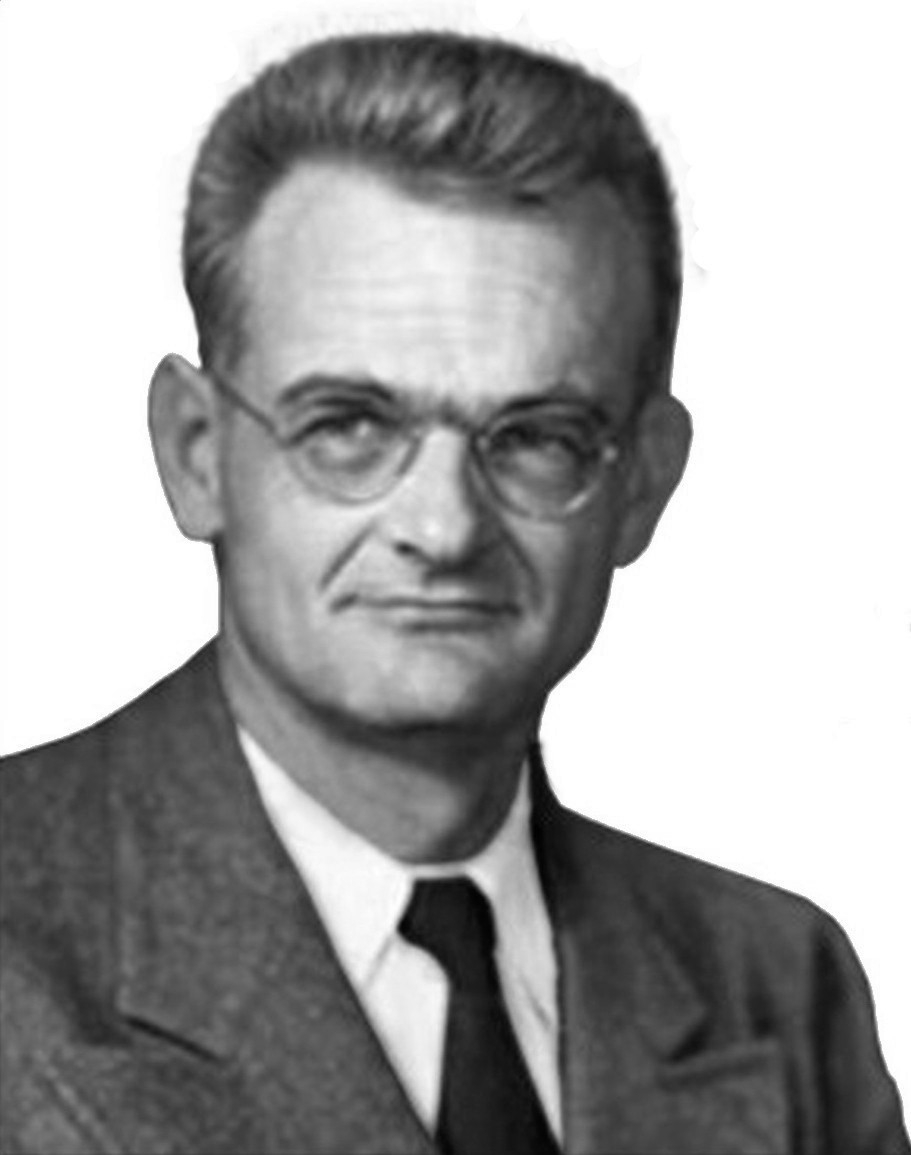
\includegraphics[width=5cm]{figures/Clarence_Zener.jpg}
%	« Clarence Zener » par Mcapdevila — {Modified:http://histo.cat/1/Clarence_Zener.jpg. Sous licence Creative Commons Attribution-Share Alike 3.0 via Wikimedia Commons - http://commons.wikimedia.org/wiki/File:Clarence_Zener.jpg#mediaviewer/File:Clarence_Zener.jpg
\begin{center}
%
\includegraphics[width=2cm]{figures/QR_zener.pdf}
\end{center}
}
{Clarence Melvin Zener et Leo Graetz}%R
	\label{Q:28}

%
\vspace{-1.25cm}
\begin{figure*}[h!]
\vspace{-1cm}
	\begin{center}
	\subfloat[Redresseur à mercure, BEAMS -- Laboratoire~d'électricité~bâtiment~L]{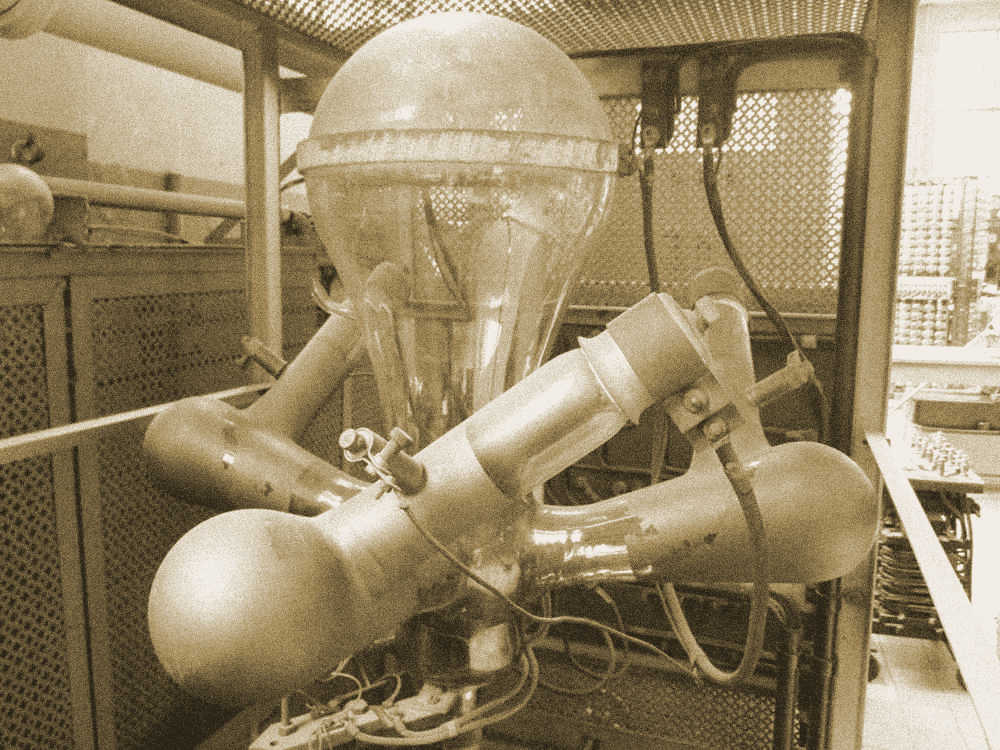
\includegraphics[width=4cm]{figures/IMG_3843rs2.jpg}}\hspace{1cm}
	\subfloat[Redresseur au Sélénium {\tiny \textit{transferred to fr.wikipedia Commons by User : Bloody-libu Public domain via Wikimedia Commons}}]{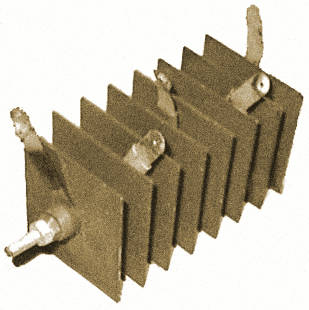
\includegraphics[width=4cm]{figures/Redresseur_Seleniums.jpg} 
	}\hspace{1cm}
	\subfloat[Diode~à~vide, BEAMS -- Laboratoire~d'électronique bâtiment~U]{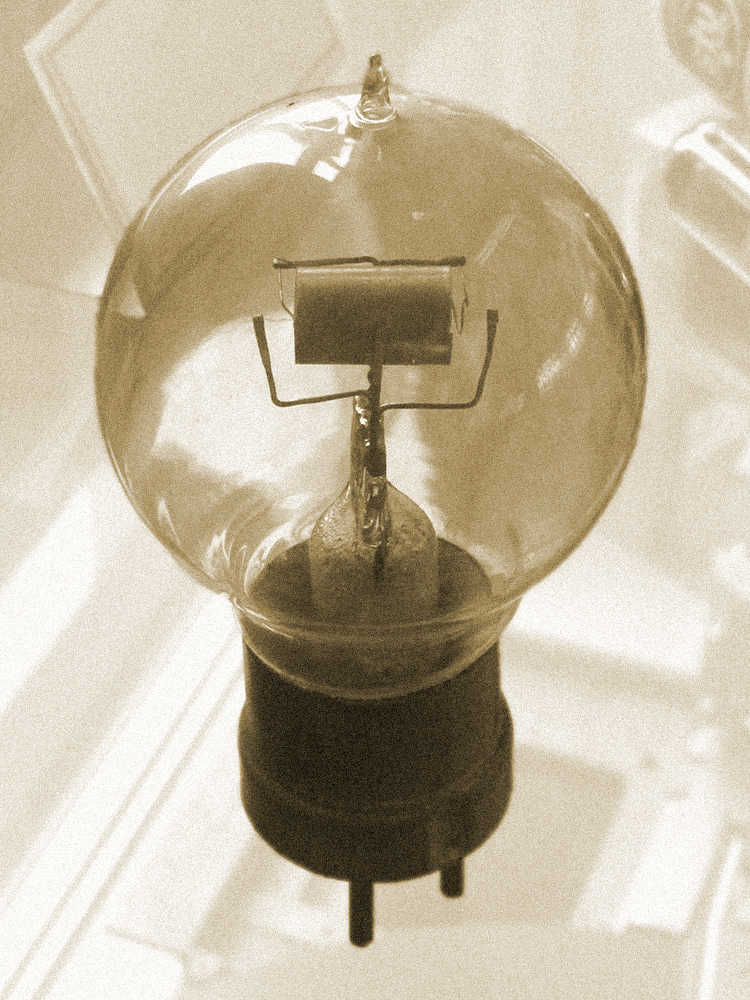
\includegraphics[width=3cm]{figures/diode_viders.jpg}}
	%		\includegraphics[width=15cm]{figures/-crop.pdf}
	\end{center}\vspace{-0.75cm}
\caption{Redresseurs d'un autre temps\dots}
\vspace{-0.5cm}
\label{fig:}
\end{figure*}
\end{document}
